\chapter{La Blockchain : un outil pour faciliter le partage et la valorisation des données}\label{chap:chapiter2}
\chaptermark{La Blockchain : un outil pour facilliter le partage et la valorisation des données}
%\minitoc

La technologie blockchain, avec ses propriétés décentralisées et sécurisées, est en train de remodeler de nombreux aspects de notre économie et de notre société. Ce chapitre débute avec une exploration approfondie de la blockchain dans la \autoref{sec:concert_crypto}, de son fonctionnement fondamental à son potentiel dans le partage de données (\ref{subsec:blockchain}, en mettant particulièrement l'accent sur les contrats intelligents (\ref{subsec:smart_contracts}).

Une fois ces bases établies, il sera procédé à l'examen de l'avènement de l'Open Knowledge Protocol For (OKP4) dans la \autoref{sec:know_era}. L'accent sera mis sur la technologie qui marque l'ère de l'économie de la connaissance. En traçant le passage de l'économie de la donnée à celle de la connaissance (\ref{subsec:economie_de_la_donnee} - \ref{subsec:economie_de_la_connaissance}), l'analyse sera axée sur le rôle du protocole OKP4. Cela fournira un aperçu de la structure (\ref{subsec:presentation_okp4} - \ref{subsec:aperçu_general_protocol}), des mécanismes de gouvernance (\ref{subsubsec:la_gouvernance_okp4}) et de l'ontologie associée (\ref{subsec:ontolologie}). L'objectif de cette section sera de guider la compréhension de la manière dont la blockchain, en conjonction avec des protocoles novateurs comme OKP4, peut redéfinir notre approche envers l'accès, la gestion et la valorisation de la connaissance.
\begin{comment}
    Après avoir établi ces bases,  dans la \autoref{sec:know_era} nous nous pencherons sur l'avènement de l'Open Knowledge Protocol For (OKP4), une technologie qui marque l'ère de l'économie de la connaissance. En traçant le passage de l'économie de la donnée à l'économie de la connaissance (\ref{subsec:economie_de_la_donnee} - \ref{subsec:economie_de_la_connaissance}), nous analyserons le rôle du protocole OKP4, en fournissant un aperçu de sa structure (\ref{subsec:presentation_okp4} - \ref{subsec:aperçu_general_protocol}), de ses mécanismes de gouvernance (\ref{subsubsec:la_gouvernance_okp4}) et de son ontologie (\ref{subsec:ontolologie}]). Cette section servira de guide pour comprendre comment la blockchain, combinée avec des protocoles innovants comme OKP4, peut redéfinir notre manière d'accéder, de gérer et de valoriser la connaissance.
\end{comment}


\section{Comprendre la blockchain}\label{sec:concert_crypto}

\subsection{La blockchain} \label{subsec:blockchain}


La blockchain, communément appelée le "grand livre numérique", est un tour de force technologique qui fait écho aux profondeurs de l'innovation. La blockchain est en fait une forme particulière de technologie de registres distribués, ou Distributed Ledger Technology (DLT) en anglais. Cette technologie, comme le souligne \citeauthor{satoshi_nakamoto_bitcoin_2008} (\citeyear{satoshi_nakamoto_bitcoin_2008}) dans son célèbre livre blanc, est une structure de données décentralisée et distribuée qui assure la transparence, la sécurité et l'immutabilité des transactions. Elle se caractérise par un système de réseau peer-to-peer où chaque participant, ou nœud, maintient, vérifie et valide les transactions. Les mécanismes de consensus, tels que la preuve de travail (Proof of Work) ou la preuve d'enjeu (Proof of Stake), ont une importance cruciale pour garantir un accord unanime parmi les nœuds sur l'état actuel de la blockchain, comme le décrit \citeauthor{vitalik_buterin_next-generation_2014} (\citeyear{vitalik_buterin_next-generation_2014}) dans le livre blanc de l'écosystème Ethereum. 

\begin{tcolorbox}
\textbf{La Blockchain simplement}

Imaginez un livre d'histoire géant, où chaque page représente un événement important. Une fois qu'une page est écrite et ajoutée au livre, elle ne peut plus être modifiée ou supprimée. C'est à peu près ce qu'est la blockchain - une série de <<pages>> ou de blocs d'information qui sont liés les uns aux autres en une chaîne permanente et immuable.

Maintenant, imaginez que chaque personne dans votre quartier a une copie exacte de ce livre d'histoire. Chaque fois qu'un nouvel événement se produit et qu'une nouvelle page doit être ajoutée, tout le monde dans le quartier doit être d'accord sur ce qui s'est réellement passé. C'est ce qu'on appelle un système <<peer-to-peer>>. Il n'y a pas de personne ou d'organisation centrale qui décide de ce qui est vrai ou non ; c'est un effort communautaire.

Alors, comment tout le monde s'accorde-t-il sur la vérité d'un nouvel événement ? C'est là qu'interviennent les mécanismes de consensus. C'est comme un ensemble de règles que tout le monde a accepté de suivre. Si un nouvel événement respecte ces règles, tout le monde convient qu'il est vrai et peut être ajouté au livre d'histoire. Une fois qu'un événement est dans le livre, il ne peut plus être modifié ou supprimé. C'est ce qui ce qui sécurise la blockchain et la rend fiable.
%\addcontentsline{toc}{subsection}{Encart 1 : La Blockchain simplement}
\end{tcolorbox}

\subsection{Les contrats intelligents}\label{subsec:smart_contracts}


Un contrat intelligent, ou smart contract, est un programme exécuté sur une blockchain qui automatise l'exécution d'actions. Il s'agit essentiellement d'un ensemble d'instructions de codées qui sont exécutées lorsqu'une condition prédéfinie est remplie. Les contrats intelligents permettent de réaliser des transactions et des accords entre parties anonymes sans avoir besoin d'un intermédiaire central, tels qu'une banque ou un avocat.

La caractéristique principale des contrats intelligents est leur nature auto-exécutable. Une fois déployé sur la blockchain, un contrat intelligent est inaltérable et s'exécute de manière autonome, sans nécessiter d'intervention humaine. Cette propriété assure un niveau élevé de confiance et de sécurité, car elle élimine la possibilité de manipulation, de fraude ou d'erreur humaine

Le concept de contrat intelligent a été introduit par \citeauthor{nick_szabo_idea_1997}, un cryptographe et informaticien, en 1994, bien avant la création de la blockchain. Cependant, ce n'est qu'avec l'avènement d'Ethereum, une plateforme blockchain dédiée à l'exécution de contrats intelligents, que le concept a pris toute son ampleur.

Les contrats intelligents ont le potentiel de révolutionner de nombreux secteurs, comme la finance, l'énergie, l'agriculture et la logistique, en automatisant les processus contractuels comme les consentements dans le partage de données.


\subsection{La Blockchain et le partage de données} \label{subsec:bc_partage}


La blockchain joue un rôle pivot dans la facilitation du partage et de la valorisation des données grâce à sa structure unique et à ses mécanismes innovants. En premier lieu, la blockchain offre une traçabilité indéniable sur les différentes opérations et transactions. Chaque action effectuée est enregistrée de manière transparente et indélébile, créant une piste d'audit fiable qui favorise la responsabilité et la confiance \footnote{Dans l'écosystème du protocole OKP4 il s'agit d'actions comme référencer un jeu de données, modifier les métadonnées d'une ressource, des informations sur les résutats d'une chaine de traitement, les flux de token, etc.}.

Ensuite, les contrats intelligents (\ref{subsec:smart_contracts}) introduisent un niveau d'automatisation et de sécurité inédit dans la gestion des consentements et le contrôle de l'accès aux données. Ces contrats codifiés exécutent automatiquement des actions lorsque certaines conditions sont remplies, éliminant ainsi la nécessité d'un intermédiaire et minimisant les risques d'erreur humaine ou de manipulation malveillante.

De plus, la blockchain peut être façonnée pour constituer un environnement économique et financier complet. Au cœur de cet environnement se trouvent des tokens ou jetons, qui jouent un rôle primordial dans la stimulation de la collaboration. Ces jetons, qui possèdent une valeur économique, peuvent être utilisés pour récompenser le partage et l'utilisation des données, créant ainsi une économie dynamique axée sur la connaissance.

En encourageant les utilisateurs à contribuer activement et à participer à l'écosystème de la blockchain, ces jetons facilitent la circulation de l'information et la création de nouvelles connaissances. En d'autres termes, la blockchain permet de monétiser les connaissances et l'expertise, donnant naissance à une économie de la connaissance.

Ainsi, en utilisant la blockchain comme outil, il est possible de créer un écosystème complet qui non seulement valorise le partage et l'utilisation des données, mais encourage également une participation active et une collaboration continue. C'est un environnement où le partage est récompensé, et où chaque contribution enrichit l'ensemble de la communauté.

Cependant, pour que la blockchain puisse véritablement faciliter le partage et la valorisation des données, elle doit être soutenue par des couches supplémentaires d'interopérabilité et d'orchestration. L'interopérabilité permet à diverses infrastructures informatiques de communiquer efficacement, quel que soit le format des données, améliorant ainsi la portée et l'efficacité du partage des données. L'orchestration assure une coordination et une gestion efficace des divers processus et transactions au sein de l'écosystème. En s'appuyant sur les règles et les consentements définis dans les contrats intelligents, elle garantit un fonctionnement fluide et sécurisé. Ces éléments, combinés à la robustesse inhérente de la blockchain, en font un outil puissant pour le partage et la valorisation des données à l'ère numérique.


\section{Open Knowledge Protocol For : L'ère de l'économie de la connaissance }\label{sec:know_era}


\subsection{L'économie de la donnée} \label{subsec:economie_de_la_donnee}


L'économie de la donnée est un concept complexe et multidimensionnel qui a évolué de manière significative ces dernières années. Elle couvre un ensemble d'activités économiques qui peuvent aller de la collecte, du stockage, du traitement à l'utilisation de données. De plus, elle intègre les transactions relatives aux données et leur exploitation pour créer de la valeur.

Dans cette économie, deux modèles principaux sont mis en évidence par \citeauthor{otto_designing_2022} (\citeyear{otto_designing_2022}). Le premier concerne la mise en commun de données similaires par différents agents économiques afin d'augmenter le volume de données. Le deuxième porte sur la mise en commun de données complémentaires pour le développement d'applications qui n'auraient pas pu être réalisées autrement. Ces modèles prônent le partage de données dans des espaces de données spécifiques. Néanmoins, ces modèles ne mettent pas suffisamment l'accent sur la rémunération des participants.

Dans la pratique il existe un troisième modèle plus répandue omis par \citeauthor{otto_designing_2022}  celui des places de marché de données (data marketplaces) où les données sont échangées contre une somme d'argent (figure \ref{fig:economie_donnée}). Ces plateformes permettent aux acteurs de vendre et d'acheter des données, généralement sous la forme de jeux de données brutes ou traitées. Cependant, ces plateformes sont souvent critiquées pour leur tarification opaque, la longue durée des négociations, la difficulté à fixer un prix juste et le manque de transparence en matière de propriété et de confidentialité des données.

\begin{figure}[h]
    \centering
    \includegraphics[width=0.8\textwidth]{ILLUSTRATIONS/data_economie.jpg}
    \caption{L'économie de la donnée}
    \label{fig:economie_donnée}
\end{figure}

%Plusieurs initiatives européennes, comme %l'International Data Spaces (IDS), iSHARE, et %i4Trust, cherchent à résoudre ces problèmes. Ces %initiatives visent à développer des %infrastructures et des écosystèmes propices au %partage sécurisé de données, tout en établissant %un cadre de confiance pour les acteurs impliqués. %Elles tentent de promouvoir une économie de la %donnée plus ouverte, plus transparente et plus %équitable.

%- échange de données => accès au données brutes
%- perte de proprité, confidentialité, souveraineté
%- Tarification opaque des données => marché très peu effiscients (McKinsey 2011)
%- Longues négociations
%- Difficulté de fixer un prix => valeur subjective et paralysie du vendeur.....

\subsection{L'économie de la connaissance} \label{subsec:economie_de_la_connaissance}


L'économie de la connaissance est un nouveau paradigme proné avec le protocole OKP4 qui replace l'alignement des intérêt au coeur du modèle économique et corrige la perte de confidentialité et de souveraineté dans les data marketplaces. En effet, dans un écosystème de partage de données, les fournisseurs de données peuvent avoir des intérêts à partager divergents. Les uns peuvent être intéressés par une contrepartie financière, les autres juste par le résultat de la coopération c'est à dire la connaissance.

\begin{figure}[h]
    \centering
    \includegraphics[width=0.8\textwidth]{ILLUSTRATIONS/kg_economie.jpg}
    \caption{L'économie de la connaissance}
    \label{fig:economie_connaissance}
\end{figure}

Dans cette économie de la connaissance, les données brutes ne sont jamais accessibles à l'utilisateur final qui n'a accès qu'à la connaissance qui est le produit d'une transformation des données des fournisseurs par des algorithmes de l'écosystèmes de partage. Cette connaissance peut être ensuite valorisée sur une \textit{data marketplace} du \textit{dataverse} ou hors de l'écosystème de partage. Les fournisseurs de données sont alors rétribués au prorata de leurs contributions (\ref{subsubsec:calcul_contrib}).

Dans le modèle d'une économie de la connaissance, les fournisseurs de données n'ont plus à s'inquiéter de la perte de souveraineté sur leurs données, puisqu'elles restent à la source et ne sont jamais accesssibles à l'utilisateur de la connaissance. Les risques et les coûts du partage de données sont donc reéquilibrés dans ce modèle avec une dimension incitative importante rendue possible par le protocole OKP4.

Dans la prochaine section nons présentons comment l'économie de la connaissance est rendue possible par le protocole OKP4.


\subsection{Présentation du protocole OKP4} \label{subsec:presentation_okp4}

Open Knowledge Protocol For (OKP4) est le protocole dédié au partage de données et de ressources numériques pour le traitement de ces données et leur valorisation en connaissances. C'est un protocole qui s'articule autour d'une blockchain BFT-POS layer-1\footnote{BFT-POS signifie Byzantine Fault Tolerant - Proof of Stake. "layer-1" se réfère à la couche principale de la blockchain, où les protocoles de consensus et les opérations de base sont exécutés.}. OKP4 fournit une solution unique aux défis inhérents au partage des ressources numériques tout en permettant l'orchestration de diverses ressources partagées \footnote{L'orchestration dans l'écosystème OKP4 désigne le déclenchement automatisé de tâches de traitement impliquant des services et des données lorsque lorsque des conditions sont atteintes.}. OKP4 facilite l'interopérabilité entre les ressources tout en garantissant le respect constant des règles de consentement associées et une auditabilité continue (\autoref{fig:respect_consentement}). Avec OKP4 naît l'économie de la connaissance (\autoref{fig:economie_connaissance}).

Le protocole OKP4 résout les problèmes du partage de données en adressant trois (03) aspects :  la confiance, des incitations à partager et la défragmention des ressources numériques.

Le protocole OKP4 s'appuie sur la technologie blockchain pour cultiver la confiance dans l'écosystème, tant pour les fournisseurs que pour les consommateurs de données et de services numériques, et élimine le besoin d'un tiers de confiance. Sa nature décentralisée assure transparence et impartialité et permet à quiconque de pouvoir l'auditer, vérifier les transactions et le respect des règles de consentements.

\begin{figure}[h]
    \centering
    \includegraphics[width=0.9\textwidth]{ILLUSTRATIONS/étapes_conso_connaissance.png}
    \caption{Le respect des consentements dans l'écosystème OKP4}
    \label{fig:respect_consentement}
\end{figure}

De plus, reconnaissant le rôle essentiel des incitations pour motiver les participants à partager leurs données et leurs connaissances, OKP4 fournit un système innovant et très flexible de compensation et de modèles économiques dans le cadre de l'économie de la connaissance. Cela permet à chaque participant de fixer leurs propres conditions de partage et le type de contrepartie qu'ils souhaitent recevoir en retour.

Enfin, OKP4 résout le problème de la fragmentation des données en proposant une solution qui permet le <<tout en tant que service>> \footnote{De l'anglissisme <<\textit{Anything as a Service (AaaS)}>>. Les ressources numériques (infrastructures, jeux de données, services, etc.) restent stockées à leurs sources et sont accessibles via une Application Programmation Interface qui permet de les utiliser comme service en ligne.}. Cette approche démantèle les silos de données isolés, permettant à toute ressource numérique d'être offerte sous forme de service. Elle améliore ainsi la découverte et l'utilisation de ressources de différentes sources et formats, et favorise la génération de nouvelles connaissances. En tant que solution technologiquement agnostique, OKP4 assure l'interopérabilité entre divers systèmes, plates-formes et technologies. Cette approche flexible et inclusive stimule l'innovation et promeut un paysage numérique plus collaboratif et efficace.

%Le protocole OKP4 vise à établir un système qui favorise la coopération, la co-innovation et le partage de savoirs tout en préservant et respectant les consentements et les intérêts personnels. En tant que bien public et neutre, OKP4 met l'accent sur des solutions techniques pour proposer une infrastructure polyvalente, sécurisée et agnostique dédiée à la résolution des problématiques humaines. Le défi réel réside dans la mise en place d'une solution qui soit assez adaptable pour répondre aux exigences des diverses parties impliquées, suffisamment expressive pour comprendre et permettre l'interopérabilité entre divers composants, et assez sûre pour fonctionner dans un environnement de confiance. Le projet OKP4 repose sur quatres piliers à savoir la décentralisation, l'interopérabilité, l'ouverture et la modularité.

\subsection{Aperçu général du protocole OKP4}\label{subsec:aperçu_general_protocol}


Le protocole OKP4 met en lien des ressources hors chaîne avec des règles et une gouvernance (\ref{subsec:rulebook}) sur mesure, qui sont consignées dans la blockchain, source de confiance inaltérable \footnote{Dans l'ecosystème OKP4, les données, services de traitement etc. restent à la source dans le système d'information du fournisseur-participant. Seules les métadonnées et les règles de gouvernance sont visibles sur la blockchain}. Cette configuration autorise chaque individu à développer des applications spécialisées, qui tirent parti de données et d'algorithmes partagés via une couche de réconciliation pérenne \footnote{Toutes les transactions peuvent être auditées en cas de conflits.}.

Trois composantes sont à distinguer dans l'écosystème du protocole OKP4 présenté sur la figure \ref{fig:architecture_protocole}:
\begin{itemize}
    \item Une source immuable de vérité et de confiance : La blockchain et son mécanisme de consensus ;
    %\item Une solution ouverte et interopérable pour partager des ressources et définir des règles pour les orchestrer : La couche protocole ;
    \item Les ressources digitales stockées à leurs sources, hors chaîne : le \textit{dataverse} ;
    \item Les applications développées sur le protocole utilisant les ressources partagées : La couche cas d'usages.
\end{itemize}

\begin{figure}[h]
    \centering
    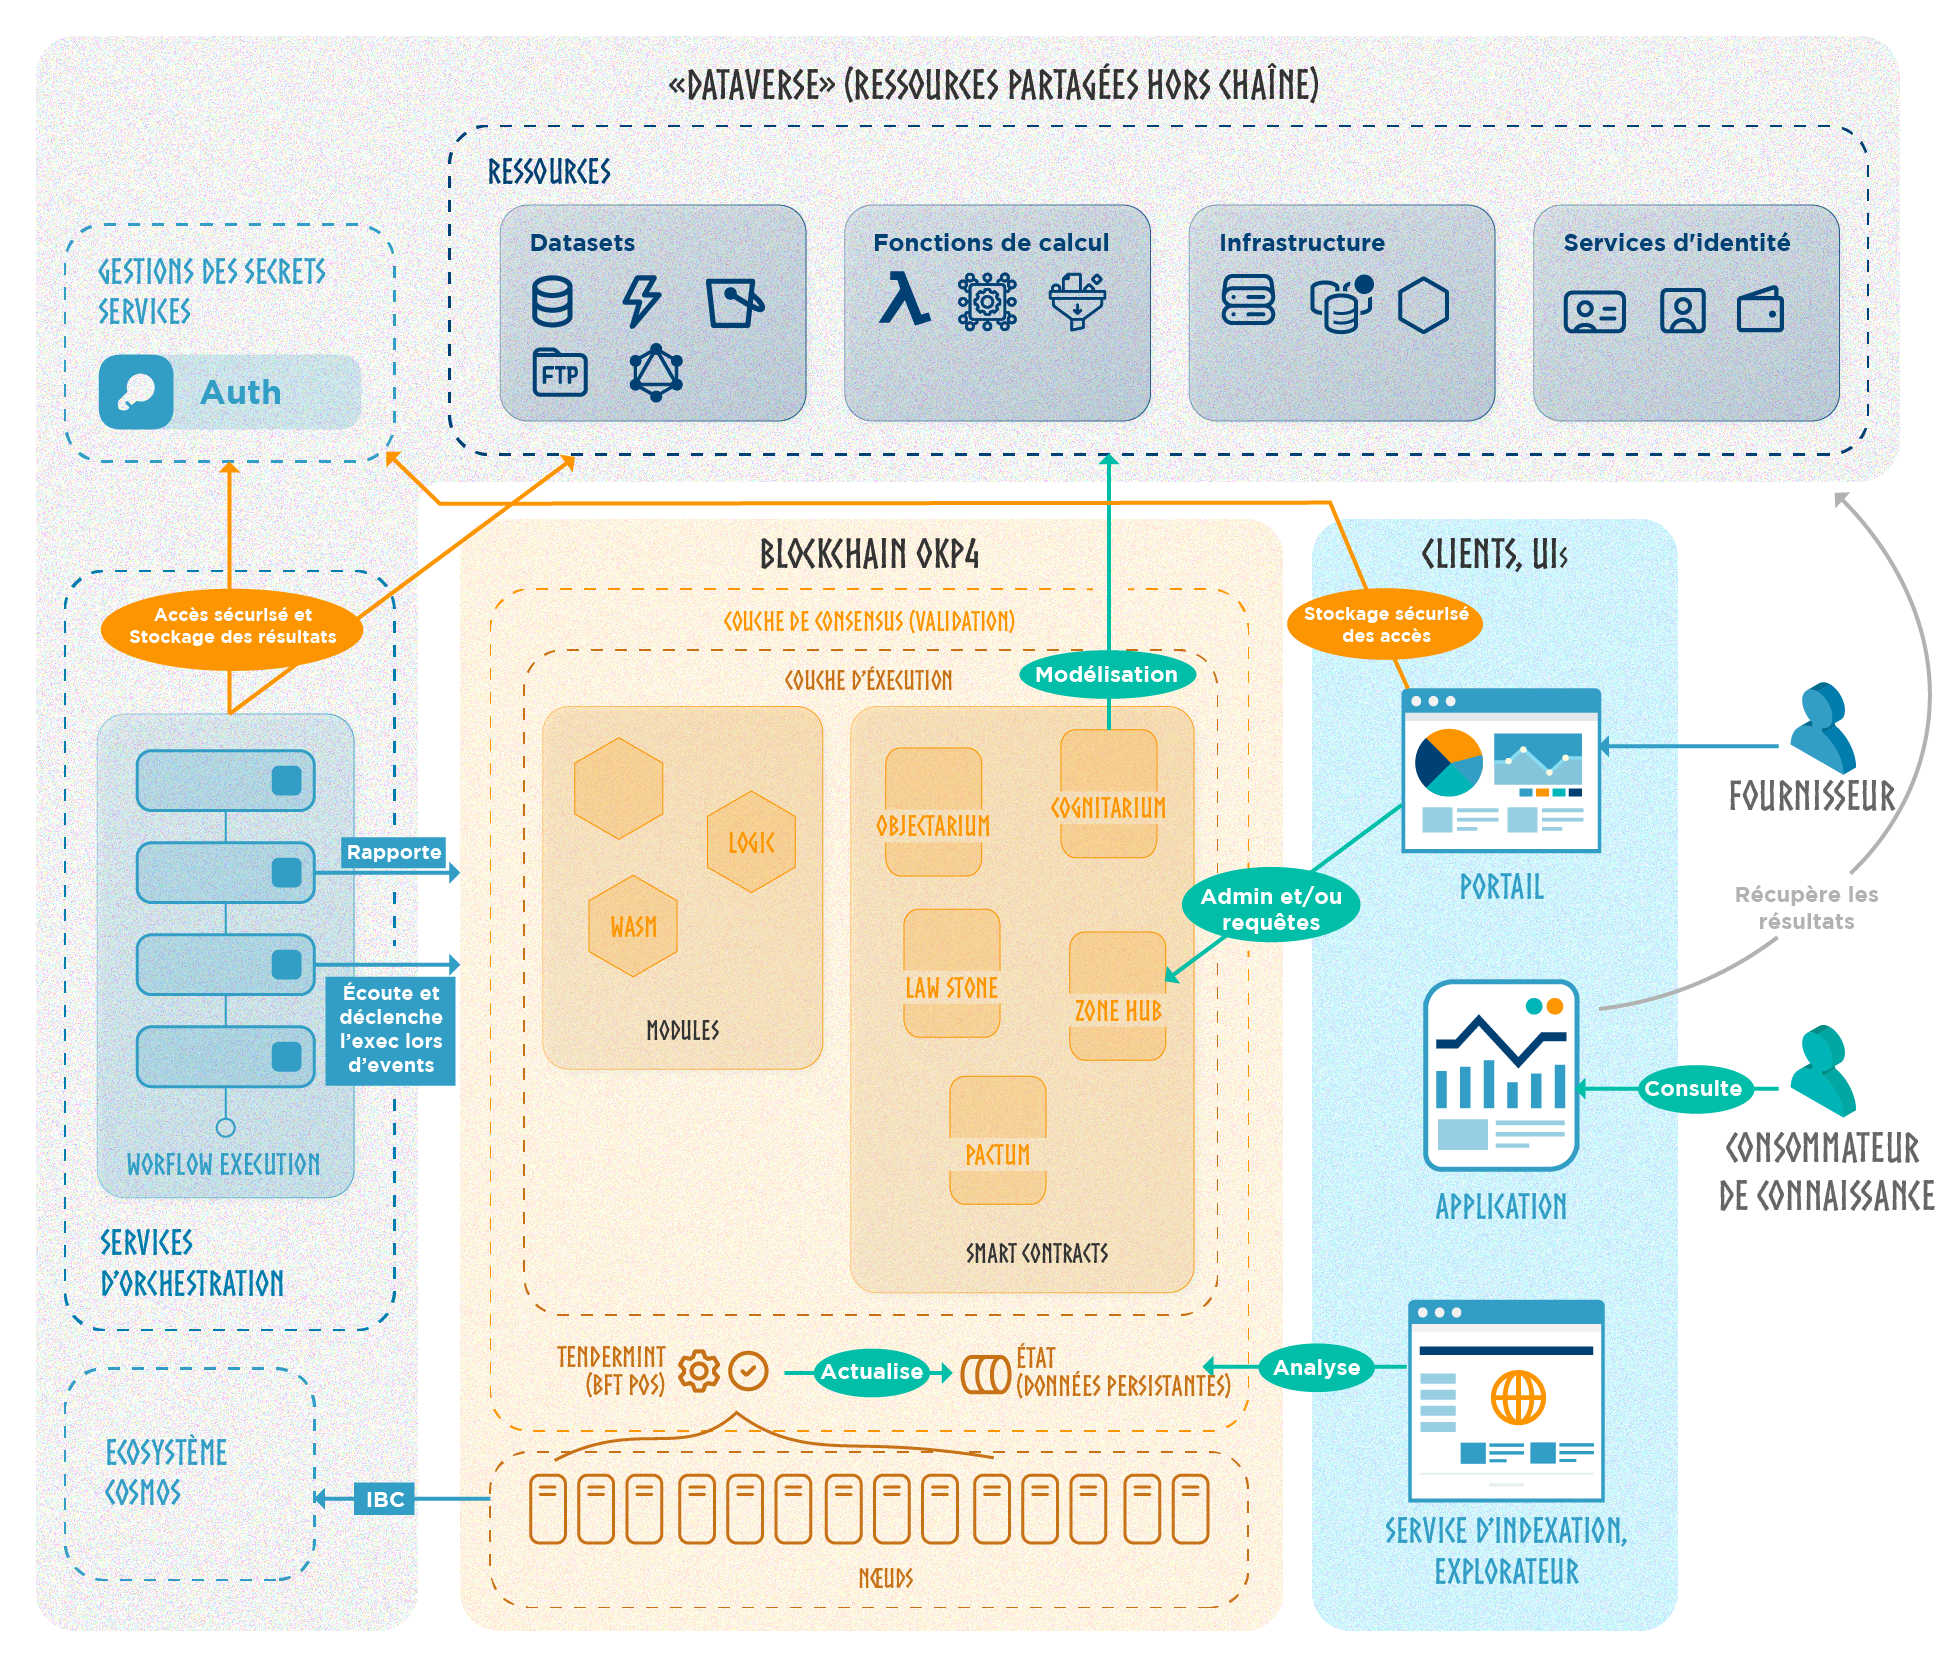
\includegraphics[width=0.8\textwidth]{ILLUSTRATIONS/architecture.png}
    \caption{Aperçu de l'architecture du protocole OKP4}
    \label{fig:architecture_protocole}
\end{figure}

\subsubsection{La blockchain et son mécanisme de consensus : La base fondamentale d'OKP4} \label{subsubsec:apercu_bc_consensus_okp4}


La couche blockchain d'OKP4, un registre distribué décentralisé public, agit comme une couche de règlement essentielle, validant et enregistrant les actions de la Couche Protocole. Cette couche offre des outils pour la création d'applications uniques. Construite sur le Cosmos SDK \footnote{Le Cosmos SDK (\textit{Software Development Kit}) est un framework open source qui permet de créer facilement et personnaliser des blockchains interopérables et évolutives.} et utilisant l'algorithme de consensus \textit{BFT du Tendermint Core}, cette chaîne \textit{Proof of Stake} est spécifiquement conçue pour répondre au mieux aux besoins du protocole.

À l'instar de toutes les blockchains, la blockchain OKP4 est constituée d'un réseau de nœuds organisés en peer-to-peer (P2P). Chaque nœud dispose d'une copie du grand livre et participe au consensus. Ces nœuds mettent en œuvre deux types de composants logiciels : les modules et les contrats intelligents. La blockchain du protocole OKP4 se démarque des autres blockchains (notamment celles de l'écosystème Cosmos) par son module Logic, ainsi que ses contrats intelligents spécifiques que sont l'Objectarium, le Law-Stone, le Cognitarium, le Zone-hub et le Pactum. Le module Logic et les contrats intelligents s'articulent autour de trois piliers fondamentaux dans le protocole : l'ontologie du protocole OKP4, la gouvernance et l'orchestration.

\begin{figure}[h]
    \centering
    \includegraphics[width=0.4\textwidth]{ILLUSTRATIONS/piliers.png}
    \caption{Les piliers du protocole OKP4}
    \label{fig:piliers_protocole}
\end{figure}


\subsubsection{\textit{dataverse} : L'Environnement Numérique} \label{subsubsec:aperçu_dataverse}


Le \textit{dataverse} est le répertoire des ressources numériques indexées et décrites dans le protocole \footnote{Les données sont décrites en \textit{Resource Description Framework} (RDF) qui est un modèle de graphe destiné à décrire formellement les ressources Web et leurs métadonnées, afin de permettre le traitement automatique de telles descriptions.}, englobant les ensembles de données, les algorithmes, le stockage, le calcul, les moteurs de flux de travail, etc. Tout élément numérique peut être partagé et référencé dans le \textit{dataverse}, permettant le \textit{Anything-as-a-Service (XaaS)}. Le \textit{dataverse} sert d'environnement hors chaîne orchestré par le protocole, où toutes les actions sont déclenchées sur la chaîne, selon les règles.

Les services d'orchestration, en écoute de la blockchain et des règles qui y sont inscrites, offrent un espace ouvert et inter-opérable adapté à toutes ressources, règles personnalisées, mécanismes de gouvernance et modèles d'affaires. Cela favorise l'alignement des intérêts parmi les participants et soutient le développement d'applications utiles basées sur des ressources partagées. La conception sans permission \footnote{De l'anglissisme \textit{"Permissionless"} qui veut dire ouvert à tous et fonctionne sur le principe de la participation ouverte et libre.} du protocole OKP4 encourage les développeurs à innover, les fournisseurs (de données, d'infrastructures et d'algorithmes) à partager, les consommateurs à utiliser, et les utilisateurs à tirer des avantages, tout en facilitant la coordination pour la création de connaissances dans le \textit{dataverse}.

\begin{figure}[h]
    \centering
    \includegraphics[width=0.7\textwidth]{ILLUSTRATIONS/dataverse_1.png}
    \caption{Le dataverse}
    \label{fig:dataverse}
\end{figure}

\subsubsection{Applications : Les cas d'usage} \label{subsubsec:aperu_cas_d'usage}


Les applications représentent des cas d'utilisation finaux rendus possibles par les divers services de la Couche Protocole - disponibilité des ressources, gouvernance, et orchestration décentralisée. Les développeurs peuvent créer des applications consommant les ressources du \textit{dataverse}, en interaction avec les utilisateurs finaux, soulignant l'application pratique du protocole et la création de valeur.


\subsection{La gouvernance avec le protocole OKP4} \label{subsubsec:la_gouvernance_okp4}


La gouvernance au sein du protocole OKP4 fait référence à l'établissement et à la mise en œuvre de règles, de politiques et de processus pour réguler l'orchestration des ressources numériques.

Le protocole OKP4 admet 4 niveaux de gouvernance : La gouvernance du protocole, les règles d'une zone spécifique, les consentements sur chaque ressource et les accords entre les participants.


\begin{figure}[h]
    \centering
    \includegraphics[width=0.7\textwidth]{ILLUSTRATIONS/governance_level.png}
    \caption{Hiérachie de la gouvernance dans l'écosystème OKP4}
    \label{fig:niveau_de_gouvernance}
\end{figure}


\subsubsection{La gouvernance au niveau de la zone :  Le rulebook} \label{subsec:rulebook}

Une zone \footnote{Dans l'écosystème OKP4, le terme "Zone" est équivalent au concept de \textit{"data space"}} est un commun numérique dans lequel les ressources référencées dans le \textit{dataverse} peuvent être partagées et orchestrées pour créer une connaissance. Les zones du \textit{dataverse}, qui se définissent par l'ensemble de leurs règles de gouvernance, les rulebooks, sont construites par le protocole à partir des ressources numériques dont les consentements attachés sont compatibles aux règles définies dans les différents rulebooks.

\begin{figure}[h]
    \centering
    \includegraphics[width=0.7\textwidth]{ILLUSTRATIONS/zone.png}
    \caption{Une zone du \textit{dataverse}}
    \label{fig:zone}
\end{figure}

Le rulebook établit les limites d'une zone spécifique du \textit{dataverse} selon sa fonction ou son objectif particulier. Le rulebook s'articule autour de de 4 catégories de règles qui gouvernent le partage et l'orchestration des ressources numériques dans la zone : La gestion des identités (décentralisées), le \textit{data management}, le \textit{services management} et le modèle économique.


\begin{figure}[h]
    \centering
    \includegraphics[width=0.9\textwidth]{ILLUSTRATIONS/composantes_rulebook.png}
    \caption{Composantes du rulebook}
    \label{fig:gouvernance_rulebook}
\end{figure}
\begin{comment}
    \begin{figure}[h]
    \centering
    %\includegraphics{}
    \caption{Exemple de règles du rulebook}
    \label{fig:exemple_rulebook}
\end{figure}
\end{comment}

\subsection{L'ontologie du protocole OKP4} \label{subsec:ontolologie}


Une ontologie \footnote{Le terme ontologie est utilisé pour désigner les ontologies informatiques} est une spécification partagée d’une conceptualisation. C’est un vocabulaire syntaxiquement décrit et sémantiquement spécifié dans le contexte d’un langage formel \footnote{Un langage formel est un ensemble de règles et de symboles précisement définis utilisés pour communiquer des idées et des instructions de manière très claire et sans ambiguïté.}, généralement un langage logique de premier ordre (Un langage logique de premier ordre est un ensemble de symboles et de règles permettant de représenter des connaissances et des raisonnements de manière formelle et précise.) comme le \textit{Web Ontology Language (OWL)}. Une ontologie se compose de concepts, de relations, de propriétés, d'axiomes et d'instances. En d'autres termes, une ontologie est un ensemble de définitions et de relations qui définissent les termes clés et les concepts au sein d'un domaine particulier.


\begin{tcolorbox}
\textbf{Ontologies - Favoriser l'Interopérabilité et le Traitement du Langage Naturel}


Les ontologies représentent une approche puissante pour organiser et structurer les connaissances d'un domaine spécifique de manière formelle. Elles présentent des avantages significatifs, notamment en favorisant l'interopérabilité des données et en améliorant le traitement automatique du langage naturel.

\textbf{1. Interopérabilité des Données}

L'ontologie facilite l'interopérabilité des données en définissant un ensemble de concepts, de propriétés et de relations standardisés au sein d'un domaine spécifique. Grâce à cette approche commune, les différents systèmes informatiques peuvent comprendre et échanger des informations de manière cohérente, indépendamment des différences de langage ou de format. Cette interopérabilité renforce la collaboration entre les applications et les organisations, permettant un partage fluide des données et une intégration plus efficace des ressources informatiques.

\textbf{2. Amélioration du Traitement du Langage Naturel}

L'ontologie joue un rôle crucial dans le traitement du langage naturel (NLP) en apportant une sémantique aux mots et aux phrases. En associant des concepts spécifiques à des termes et en établissant des relations entre ces concepts, l'ontologie permet aux machines de comprendre le contexte et la signification des données textuelles. Ainsi, les systèmes NLP peuvent analyser et interpréter les requêtes des utilisateurs de manière plus précise, améliorant ainsi la qualité des réponses fournies par les chatbots, les assistants virtuels et autres applications interactives.

En somme, les ontologies se révèlent être des outils essentiels pour résoudre les problèmes d'interopérabilité des données et pour améliorer le traitement du langage naturel. En établissant une base de connaissances commune et en dotant les données de sens, l'ontologie ouvre la voie à une collaboration accrue entre les systèmes informatiques et à des interactions plus intuitives avec les utilisateurs, propulsant ainsi l'ingénierie informatique vers de nouveaux horizons d'efficacité et d'innovation.


\end{tcolorbox}

Les ressources numériques partagées avec le protocole OKP4 ne sont pas directement rattachées à une Zone spécifique mais plutôt sont jugées compatibles avec certaines zones en fonction des règles de gouvernance de ces zones et des consentements attachés aux ressources. En d'autres termes, c'est le protocole qui interprète les consentements sur les ressources et les règles de gouvernance des différentes Zones puis fait le rapprochements entre zones et ressources compatibles.

\begin{figure}
    \centering
    \includegraphics[width=0.9\textwidth]{ILLUSTRATIONS/rattachement_zone.png}
    \caption{Processus de rattachement d'une ressource à une zone}
    \label{fig:rattachement_d'une_ressource}
\end{figure}

Le protocole doit donc être capable d'interpréter et représenter les règles de gouvernance et consentements. Mieux, il doit comprendre leurs dépendances et leurs hiérarchies. 

L'ontologie du protocole OKP4, est l'outil qui permet de parvenir à cette fin. L'ontologie sert à modéliser le réseau sémantique de toutes les entités du \textit{dataverse} (zones, données, services, règles, etc.) en définissant ce qu'elles sont et comment elles sont liées les unes aux autres.

\begin{comment}
    \begin{figure}
    \centering
    %\includegraphics{}
    \caption{Caption}
    \label{fig:ontologie_schema}
\end{figure}
\end{comment}

L'ontologie du protocole OKP4 est directement implémentée dans un contrat intelligent sur la blockchain : Le \textit{Cognitarium}. Cela permet l'expressivité du protocole et facilite sa compréhension structurée. 

\newpage
%\thispagestyle{empty}
%\null
%\newpage